\begin{figure}[t]
\centering
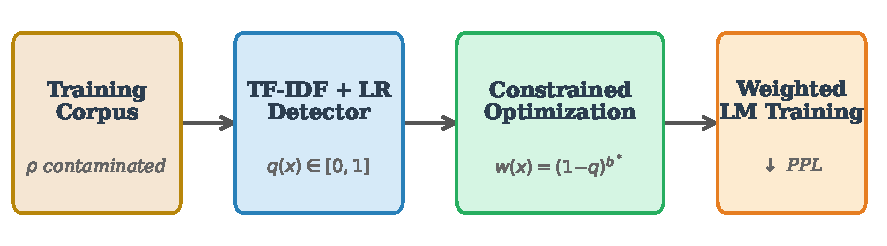
\includegraphics[width=\columnwidth]{dr_pipeline_concept}
\caption{Overview of the detect-and-reweight pipeline. A TF-IDF + LR detector assigns contamination scores $q(x)$; a dual-constrained optimizer selects $b$ to satisfy quality-floor and effective-sample-size constraints; the resulting weights $w(x) = (1{-}q(x))^{b}$ are applied during training.}
\label{fig:pipeline}
\end{figure}

Figure~\ref{fig:pipeline} illustrates the pipeline. Let $\mathcal{D}$ denote a pretraining corpus with unknown synthetic contamination ratio $\rho$~\citep{cheng2025contamination}.
A detector assigns each sample $x$ a synthetic probability $q(x) \in [0,1]$; following \citet{drayson2025detection}, we weight each sample as $w(x) = (1 - q(x))^{b}$, where $b \geq 0$ is a sharpening exponent ($b{=}0$ recovers uniform training).
Rather than selecting $b$ via grid search, we derive $b$ per-batch from the batch's $q$-score distribution using two opposing constraints.

Given a batch $\mathcal{B} = \{x_1, \ldots, x_B\}$ with scores $q_i = q(x_i)$ and weights $w_i(b) = (1 - q_i)^{b}$:

\paragraph{Quality floor.}
The \emph{effective authenticity} $\aeff(b) = \sum_i w_i(b)(1{-}q_i) / \sum_i w_i(b)$ measures the weighted mean detector confidence that samples are real.
We require $\aeff(b) \geq \tau$, yielding a lower bound $b_\tau$ on the exponent, motivated by convergence theory under contamination~\citep{wang2026survive}.
$\aeff$ correlates with the true batch-level real fraction at Pearson $r \approx 0.79$ (Appendix~\ref{app:alpha_validation}); limitations are discussed in \S\ref{sec:discussion}.

\paragraph{Stability ceiling.}
Kish's effective sample size $\mathrm{ESS}(b) = (\sum_i w_i)^2 / \sum_i w_i^2$~\citep{kish1965survey} decreases monotonically in $b$ (Appendix~\ref{app:proofs}).
We require $\mathrm{ESS}(b) \geq \nmin$, yielding an upper bound $\bess$.

\paragraph{Adaptive $\bstar$.}
Since $\aeff$ is non-decreasing and ESS is decreasing in $b$, the two constraints define an interval $[b_\tau, \bess]$.
The optimal exponent implements \emph{minimum intervention}:
\begin{equation}
  b^{*} = \begin{cases}
    0        & \text{if } \aeff(0) \geq \tau, \\
    b_\tau   & \text{if } b_\tau \leq \bess, \\
    \bess & \text{otherwise (stability precedence)},
  \end{cases}
  \label{eq:bstar}
\end{equation}
applying the smallest $b$ that achieves the quality floor.
Each batch falls into one of three regimes (clean, $\aeff$-binding, or ESS-binding; Figure~\ref{fig:dual_constraint}) whose frequencies we analyze in \S\ref{sec:regime}.
The resulting $\bstar$ trajectory (Figure~\ref{fig:bstar_traj}, Appendix) varies substantially across batches, with all three regimes alternating throughout; this per-batch variation indicates adaptation to local composition rather than global dynamics.

\begin{figure*}[t]
\centering
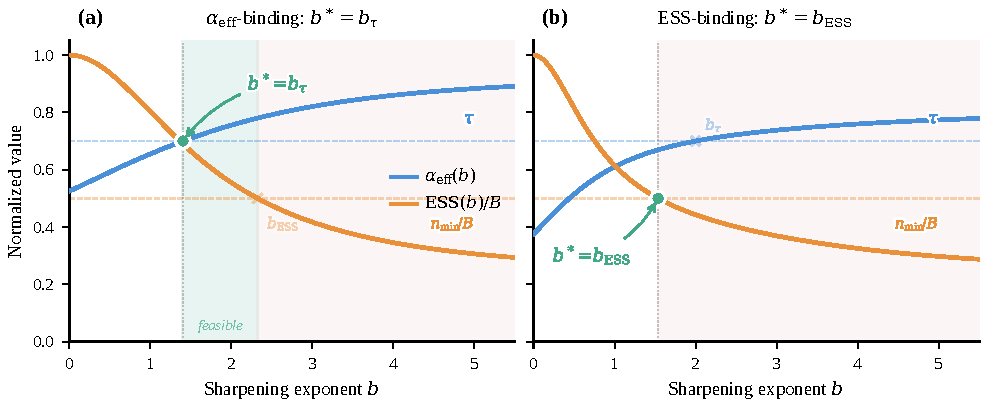
\includegraphics[width=\textwidth]{dual_constraint_illustration}
\caption{Dual-constraint $\bstar$ selection for two representative batches ($B{=}4$, $\tau{=}0.7$, $\nmin{=}2$).
\textbf{(a)}~Quality constraint binds: $\aeff(b)$ reaches $\tau$ before $\mathrm{ESS}(b)$ drops below $\nmin$, so $\bstar = \btau$.
\textbf{(b)}~Stability constraint binds: $\mathrm{ESS}(b)$ hits the floor first, so $\bstar = \bess$.
Green: feasible interval; red: over-sharpening.}
\label{fig:dual_constraint}
\end{figure*}

Given $\bstar$, normalized weights $\pi_i = w_i(\bstar) / \sum_j w_j(\bstar)$ define the weighted loss $\mathcal{L} = \sum_i \pi_i \ell_i$; $\bstar$ is found via bisection (Algorithm~\ref{alg:bstar}, Appendix~\ref{app:algorithm}) in $\mathcal{O}(B \log(b_{\max}/\varepsilon))$ operations, negligible beside the forward pass.
Defaults: $\tau{=}0.7$, $\nmin{=}\lfloor B/2 \rfloor$; sensitivity in \S\ref{sec:sensitivity}.

